% Review II Presentation -- Payload-Aware Two-Tier UAV Route Planning
% Built on the department UG Project Presentation Template.
% Compile with: pdflatex BID_Review_II_Presentation.tex  (Overleaf: upload this file + the figures/ folder)

\documentclass[aspectratio=169,11pt]{beamer}

% ---------- Theme and colours ----------
\usetheme{Madrid}
\usecolortheme{default}
\definecolor{UniversityBlue}{RGB}{16,62,110}
\definecolor{AccentBlue}{RGB}{30,136,229}
\definecolor{LightBlue}{RGB}{232,242,252}
\definecolor{DarkGray}{RGB}{55,65,81}

\setbeamercolor{structure}{fg=UniversityBlue}
\setbeamercolor{palette primary}{bg=UniversityBlue,fg=white}
\setbeamercolor{palette secondary}{bg=AccentBlue,fg=white}
\setbeamercolor{frametitle}{bg=UniversityBlue,fg=white}
\setbeamercolor{block title}{bg=UniversityBlue,fg=white}
\setbeamercolor{block body}{bg=LightBlue,fg=black}
\setbeamercolor{alerted text}{fg=AccentBlue}

% ---------- Packages ----------
\usepackage[T1]{fontenc}
\usepackage[utf8]{inputenc}
\usepackage{lmodern}
\usepackage{graphicx}
\usepackage{booktabs}
\usepackage{array}
\usepackage{tabularx}
\usepackage{tikz}
\usetikzlibrary{positioning}
\usepackage{amsmath}
\usepackage{listings}
\usepackage{xcolor}
\usepackage{colortbl}
\usepackage{hyperref}
\usepackage{pgfplots}
\pgfplotsset{compat=1.17}

\graphicspath{{figures/}}

% ---------- General settings ----------
\setbeamertemplate{navigation symbols}{}
\setbeamertemplate{caption}[numbered]
\setbeamertemplate{itemize item}{\color{AccentBlue}$\blacktriangleright$}
\setbeamertemplate{itemize subitem}{\color{UniversityBlue}$\bullet$}
\setbeamersize{text margin left=0.7cm,text margin right=0.7cm}

% Footer: project title, institution and slide number
\setbeamertemplate{footline}{%
  \leavevmode%
  \hbox{%
    \begin{beamercolorbox}[wd=.42\paperwidth,ht=2.7ex,dp=1.1ex,leftskip=.6em]{author in head/foot}%
      \insertshorttitle
    \end{beamercolorbox}%
    \begin{beamercolorbox}[wd=.46\paperwidth,ht=2.7ex,dp=1.1ex,center]{date in head/foot}%
      Department of Computer Science and Engineering
    \end{beamercolorbox}%
    \begin{beamercolorbox}[wd=.12\paperwidth,ht=2.7ex,dp=1.1ex,center]{page number in head/foot}%
      \insertframenumber/\inserttotalframenumber
    \end{beamercolorbox}%
  }%
  \vskip0pt%
}

% ---------- Code style ----------
\lstset{
  basicstyle=\ttfamily\scriptsize,
  keywordstyle=\color{UniversityBlue}\bfseries,
  commentstyle=\color{gray},
  stringstyle=\color{AccentBlue},
  numbers=left,
  numberstyle=\tiny\color{gray},
  frame=single,
  breaklines=true,
  showstringspaces=false
}

% ---------- Helpers ----------
% Highlight number box: \stat[width]{value}{label}
% Height and value size can be reduced per slide with \setlength{\statheight}{..}
% and \renewcommand{\statvalue}{\large}.
\newlength{\statheight}\setlength{\statheight}{1.45cm}
\newcommand{\statvalue}{\Large}
\newcommand{\stat}[3][0.30\textwidth]{%
  {\setlength{\fboxsep}{4pt}%
  \fcolorbox{UniversityBlue}{LightBlue}{%
    \parbox[c][\statheight][c]{#1}{\centering
      {\statvalue\bfseries\color{UniversityBlue}#2}\par\vspace{1mm}
      {\scriptsize\linespread{0.95}\selectfont #3\par}}}}}
% Smaller block titles for side-by-side blocks so the title bars do not overflow
\newcommand{\compactblocks}{\setbeamerfont{block title}{size=\small}}
% Figure caption text (keeps the report's figure numbers)
\newcommand{\figcap}[1]{\par\vspace{1mm}{\scriptsize\color{DarkGray}#1}\par}

% ---------- Project details ----------
\title[Payload-Aware Two-Tier UAV Route Planning]{Payload-Aware Two-Tier UAV\\Route Planning for Last-Mile Delivery}
\subtitle{Review Report -- II}
\author[Thirumurugan, Meghna, Shrika]{%
  Thirumurugan RA (3122235001149)\\
  Meghna Manimaran (3122235001079)\\
  Shrika SP Thota (3122235001125)
}
\institute[SSN College of Engineering]{%
  Guided by: Dr. N. Sujaudeen, Assistant Professor\\[2mm]
  Department of Computer Science and Engineering\\
  Sri Sivasubramaniya Nadar College of Engineering
}
\date{Academic Year 2026--2027}

\begin{document}

% ======================================================================
% 1. Title slide
\begin{frame}[plain]
  \titlepage
\end{frame}

% ======================================================================
% 2. First Review Queries
\begin{frame}{First Review -- Queries and Answers}
  \compactblocks
  \small
  The panel raised one concern with two parts at Review I:
  \vspace{2mm}

  \begin{columns}[T,onlytextwidth]
    \column{0.47\textwidth}
      \begin{block}{Query 1}
        The overall technical complexity of the proposed system was too low for a final-year project.
      \end{block}
    \column{0.47\textwidth}
      \begin{block}{Query 2}
        Given that complexity, a Phase I that runs until December could not be justified.
      \end{block}
  \end{columns}
  \vspace{3mm}

  Both are fair readings of the Review I prototype. Since then, the airspace graph and cost model
  --- the foundation every later stage depends on --- have been rebuilt.
  \vspace{3mm}

  \textbf{Query 1 $\rightarrow$ A richer 3-D airspace lattice and a directional wind-risk model (next slide)}\\[2mm]
  \textbf{Query 2 $\rightarrow$ Two coupled, repeated loops --- benchmarking/evaluation and simulation fidelity --- remain (slide after)}
\end{frame}

% ======================================================================
% 3. Query 1
\begin{frame}{Query 1 --- A Harder Airspace Graph \& Wind Model}
  \compactblocks
  \scriptsize
  {\footnotesize Two changes account for most of the added complexity since Review I:}
  \vspace{1mm}

  \begin{columns}[T,onlytextwidth]
    \column{0.47\textwidth}
      \begin{block}{1. Multi-source node selection}
        \begin{itemize}
          \item 3-D lattice (200 m spacing, 6 km box) replaces OSM road-only graph --- 900 candidate nodes
          \item Elevation from a 4-provider DEM chain; building heights from OSM footprints
          \item Legal ceiling check: $\max(60\,\text{m},\, h_{\text{bldg}}+15\,\text{m}) \le 120\,\text{m}$ (Drone Rules, 2021)
          \item Restricted-zone polygons remove nodes and clipping edges
        \end{itemize}
      \end{block}
    \column{0.47\textwidth}
      \begin{block}{2. Directional wind-aware risk}
        \begin{itemize}
          \item Wind split per edge into headwind + crosswind components
          \item 11-component weighted risk score (wind, gust, turbulence, rain, visibility, population, buildings\ldots)
          \item Weather gate holds all flights outside safe limits
          \item Edge costs become directional: $u\to v \neq v\to u$ under wind
        \end{itemize}
      \end{block}
  \end{columns}
  \vfill

  \centering
  \stat{+27.8\%}{energy for east-bound vs west-bound edges, 25 km/h east wind}\hfill
  \stat{6$\times$}{higher crosswind risk on N--S edges vs E--W edges (0.225 vs 0.038)}\hfill
  \stat{36 $\rightarrow$ 6--15}{routes on the Pareto front as calm air turns into a steady wind}
\end{frame}

% ======================================================================
% 4. Module 1 figures
\begin{frame}{Module 1 in Detail: Node Selection \& Wind Decomposition}
  \centering
  \begin{minipage}[t]{0.32\textwidth}
    \centering
    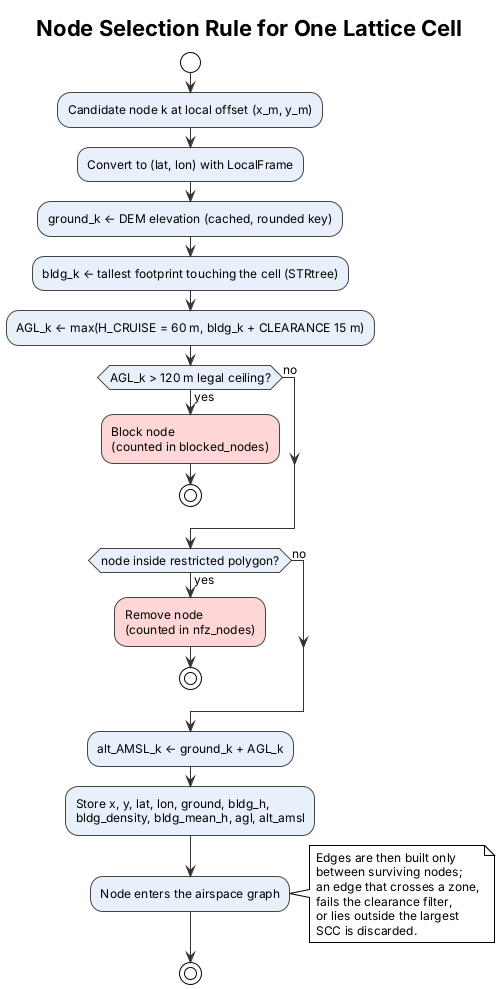
\includegraphics[height=0.66\textheight,keepaspectratio]{fig4_5_node_selection.png}
    \figcap{Fig. 4.5 -- Selection rule applied to each candidate lattice node}
  \end{minipage}\hspace{4mm}
  \begin{minipage}[t]{0.52\textwidth}
    \centering
    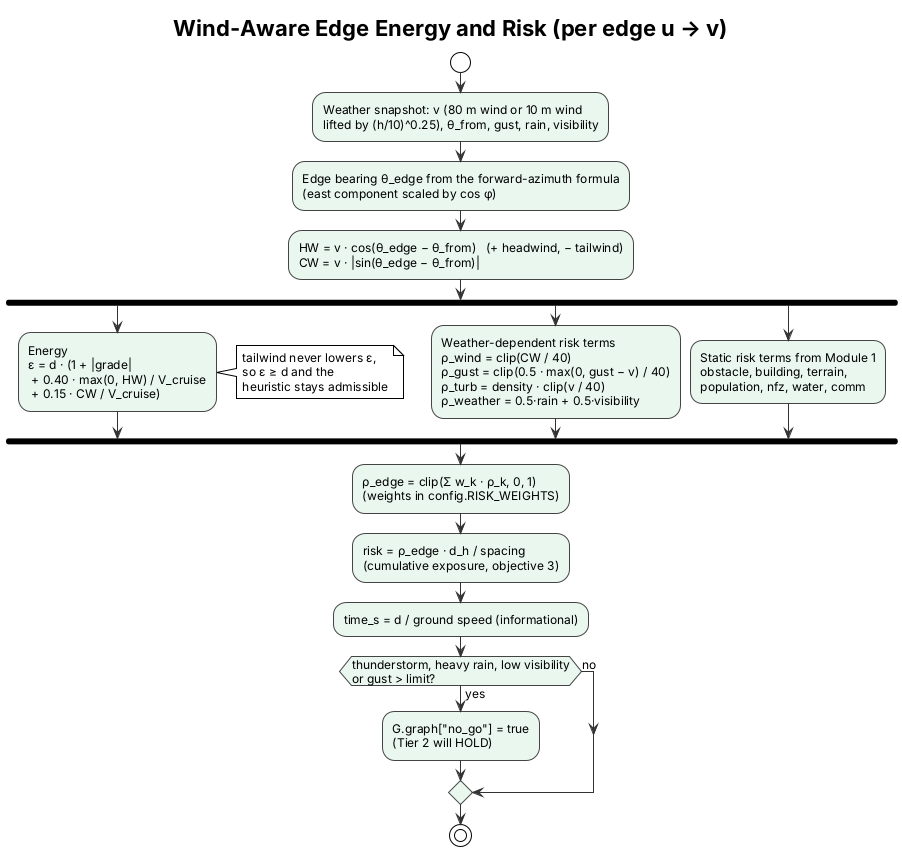
\includegraphics[height=0.66\textheight,keepaspectratio]{fig4_6_wind_decomposition.png}
    \figcap{Fig. 4.6 -- Per-edge wind decomposition into energy and risk}
  \end{minipage}
\end{frame}

% ======================================================================
% 5. Query 2
\begin{frame}{Query 2 --- Why Phase I Runs Through December}
  \compactblocks
  \scriptsize
  {\footnotesize Two pieces of work remain, and neither is a one-off task --- both are repeated loops.}
  \vspace{1mm}

  \begin{columns}[T,onlytextwidth]
    \column{0.47\textwidth}
      \begin{block}{Loop A --- Benchmark, Evaluate, Improve}
        \begin{itemize}
          \item 36 cases: 4 graphs $\times$ 9 wind directions
          \item NAMOA*, 3 single-objective A*, weighted-sum A*, and MOPSO (100 particles $\times$ 200 iters $\times$ 30 seeded reps) per case --- $\sim$21.6M particle updates/pass
          \item 225 payload-tag combinations $\times$ 4 selection rules per case
          \item First pass already surfaced 5 issues needing a fix + full re-run (density-label bug, monotonicity bug, pooled MOPSO stats, front-collapse question, placeholder weights)
          \item HV gap vs MOPSO on 200-node graph is only 0.0004 --- needs 30 reps + a statistical test before any claim is safe
        \end{itemize}
      \end{block}
    \column{0.47\textwidth}
      \begin{block}{Loop B --- Simulation Fidelity}
        \begin{itemize}
          \item SITL mission chain already flies correctly (cross-track RMS 0.11--0.13 m) --- but only with ArduPilot's built-in physics, not the city model
          \item Gazebo world must be built from live OSM + DEM and pass load/rest/real-time gates
          \item Gazebo has no wind yet, while the planner already plans for wind
          \item Battery model constants are placeholders --- must be calibrated from simulated flights per payload class
          \item Every mismatch between planned and flown route feeds back into Loop A --- the two loops are coupled and must run side by side
        \end{itemize}
      \end{block}
  \end{columns}
\end{frame}

% ======================================================================
% 6. Benchmark cycle figure
\begin{frame}{The Benchmark -- Evaluate -- Improve Cycle (Oct--Dec)}
  \centering
  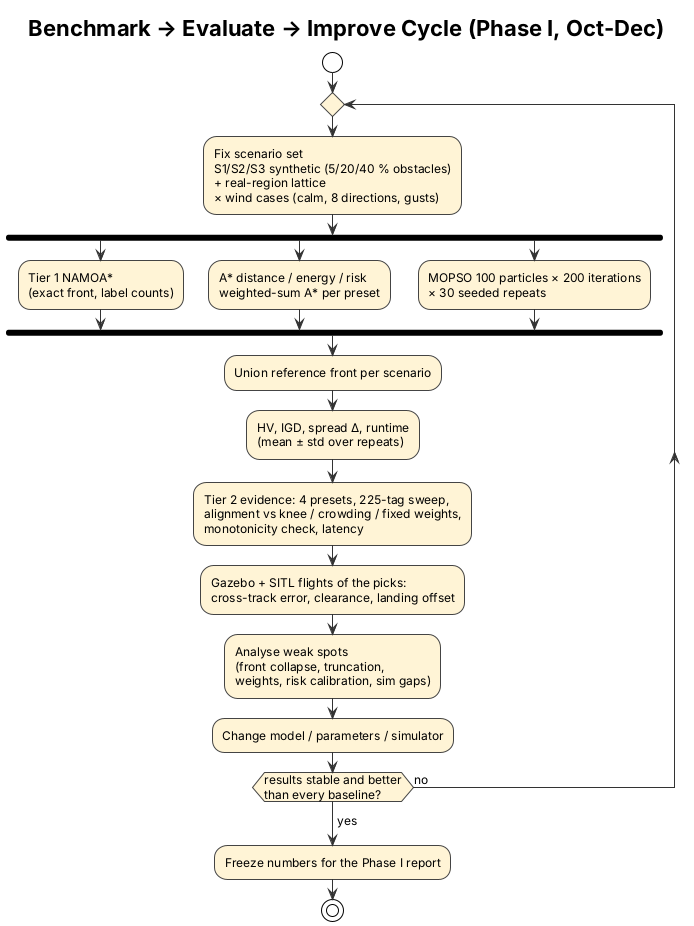
\includegraphics[height=0.72\textheight,keepaspectratio]{fig2_1_benchmark_cycle.png}
  \figcap{Fig. 2.1 -- The benchmark, evaluate and improve cycle planned for October to December}
\end{frame}

% ======================================================================
% 7. Problem statement
\begin{frame}{Problem Statement}
  \footnotesize
  \begin{alertblock}{The Problem}
    Existing UAV planners apply a fixed geometric Pareto-selection rule, or a hand-tuned weighted-sum scalar,
    independent of payload type. When the payload changes --- fragile sample vs.\ emergency medicine vs.\ bulk
    relief --- an expert must re-tune weights and re-run the search from scratch. That intervention is
    infeasible in the field.
  \end{alertblock}
  \vspace{1mm}

  \textbf{Formally}
  \begin{itemize}
    \item Given: an airspace graph $G$ with edge costs $c(e) = [\text{distance}, \text{energy}, \text{risk}]$;
          a pre-computed Pareto front $P$ over $G$; and a payload tuple $(F, W, U, P_{\text{lvl}})$ ---
          fragility, weight class, urgency, priority
    \item Select the route $p^* \in P$ that best satisfies the payload's implied routing requirements
    \item Without expert re-tuning, and without re-running the multi-objective search
  \end{itemize}
  \vspace{1mm}

  \textbf{Constraints \& success criteria}
  \begin{itemize}
    \item Selection must be deterministic, reproducible, and complete within 1 second of tag entry
    \item The selected route's distance/energy/risk must match what the payload tag implies --- checked by a Tier 2 alignment metric
  \end{itemize}
\end{frame}

% ======================================================================
% 8. Objectives
\begin{frame}{Project Objectives}
  \small
  \begin{enumerate}
    \setlength{\itemsep}{2mm}
    \item Formulate multi-objective UAV route planning as a Pareto front pre-computation task, distinguishing deterministic graph-search from stochastic population-based alternatives
    \item Design a payload metadata schema and rule-based mapping from mission context to Pareto-point selection weights, with no expert tuning
    \item Benchmark Tier 1 route quality and front coverage against single-objective A* and MOPSO using hypervolume, spread and IGD
    \item Quantify Tier 2 selection accuracy via payload-alignment across mission types (fragile sample, emergency medicine, disaster relief)
    \item Establish novelty: payload metadata as the sole, deterministic input to Pareto-point selection, replacing context-blind entropy/diversity criteria
  \end{enumerate}
\end{frame}

% ======================================================================
% 9. Architecture
\begin{frame}{Proposed System Architecture}
  \compactblocks
  \centering
  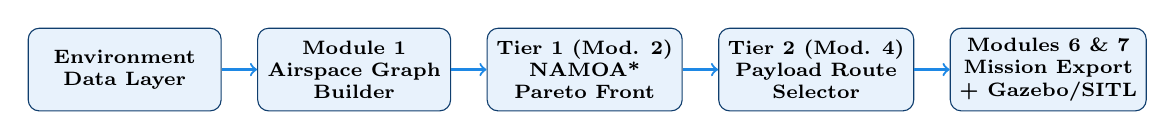
\begin{tikzpicture}[node distance=0.45cm,
      box/.style={draw=UniversityBlue,fill=LightBlue,rounded corners,
                  minimum width=2.45cm,minimum height=1.05cm,align=center,font=\scriptsize\bfseries},
      arrow/.style={->,thick,draw=AccentBlue}]
    \node[box] (env) {Environment\\Data Layer};
    \node[box,right=of env] (m1) {Module 1\\Airspace Graph\\Builder};
    \node[box,right=of m1] (t1) {Tier 1 (Mod. 2)\\NAMOA*\\Pareto Front};
    \node[box,right=of t1] (t2) {Tier 2 (Mod. 4)\\Payload Route\\Selector};
    \node[box,right=of t2] (m6) {Modules 6 \& 7\\Mission Export\\+ Gazebo/SITL};
    \draw[arrow] (env) -- (m1);
    \draw[arrow] (m1) -- (t1);
    \draw[arrow] (t1) -- (t2);
    \draw[arrow] (t2) -- (m6);
  \end{tikzpicture}
  \vspace{2mm}

  \scriptsize
  \begin{columns}[T,onlytextwidth]
    \column{0.47\textwidth}
      \begin{block}{Module 3 --- Baseline Planners}
        Single-objective A* $\times$ 3, weighted-sum A*, MOPSO --- run beside the main path for comparison
      \end{block}
    \column{0.47\textwidth}
      \begin{block}{Module 5 --- Evaluation \& Benchmarking}
        Hypervolume, IGD, spread, Tier 2 alignment, 225-tag sweep, ablation --- scores every stage
      \end{block}
  \end{columns}
  \vspace{2mm}

  \raggedright
  {\footnotesize\textbf{Key idea: the Pareto front is built once per region and weather window (Tier 1) and reused across missions; a new mission runs only Tier 2, in well under a second.}}
  \vspace{1mm}

  \begin{block}{Hard constraints enforced throughout}
    Cruise $\ge$ 60 m above ground \& 15 m above roofs $\bullet$ $\le$ 120 m AGL (Drone Rules, 2021)
    $\bullet$ no entry into restricted zones $\bullet$ route energy within 80\% of battery capacity
  \end{block}
\end{frame}

% ======================================================================
% 10. Architecture figure
\begin{frame}{System Architecture (Fig. 4.2)}
  \centering
  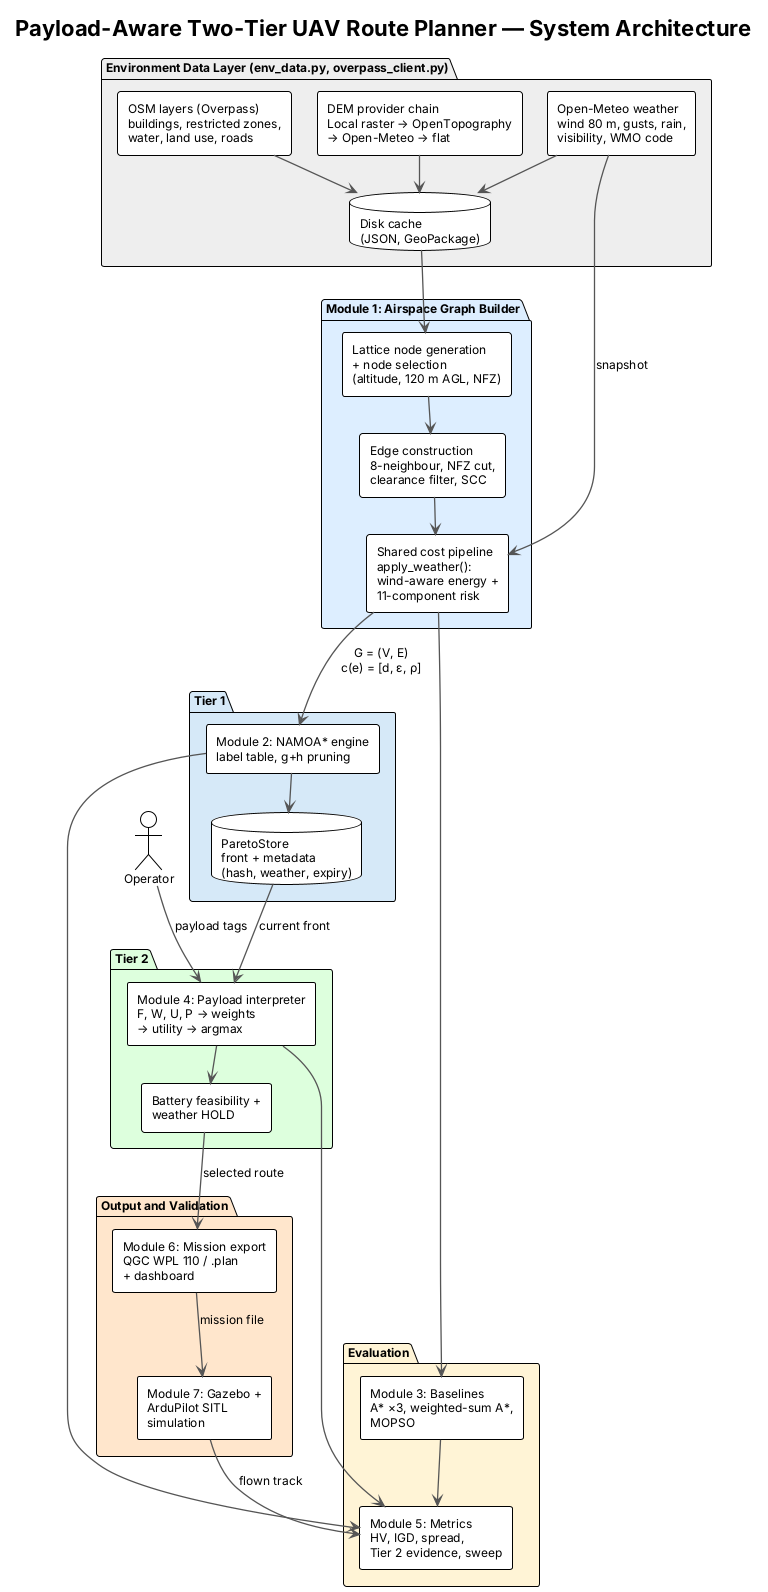
\includegraphics[height=0.70\textheight,keepaspectratio]{fig4_2_system_architecture.png}
  \figcap{Fig. 4.2 -- System architecture: Tier 1 builds and stores the front per region and weather window; Tier 2 selects a route per payload tag}
\end{frame}

% ======================================================================
% 11. Modules
\begin{frame}{System Modules}
  \footnotesize
  \begin{enumerate}
    \setlength{\itemsep}{1.2mm}
    \item \textbf{Module 1 -- Airspace Graph Builder:} 3-D lattice from DEM, OSM buildings, restricted zones; shared [distance, energy, risk] cost pipeline
    \item \textbf{Module 2 -- Tier 1 --- NAMOA* Engine:} Exact multi-objective A* search with a label table and admissible vector heuristic
    \item \textbf{Module 3 -- Baseline Planners:} Single-objective A* $\times$3, weighted-sum A*, and a MOPSO baseline
    \item \textbf{Module 4 -- Tier 2 --- Payload Selector:} Maps 4 payload tags $\rightarrow$ weights $\rightarrow$ one route; battery feasibility + weather HOLD
    \item \textbf{Module 5 -- Evaluation \& Benchmarking:} HV, IGD, spread, Tier 2 alignment, 225-tag sweep, ablation studies
    \item \textbf{Module 6 -- Mission Export \& Dashboard:} QGC WPL 110 / .plan export; Tkinter operator dashboard
    \item \textbf{Module 7 -- Simulation \& SITL Validation:} Gazebo Harmonic + ArduPilot SITL; cross-track error, clearance, landing offset
  \end{enumerate}
\end{frame}

% ======================================================================
% 12. Methodology
\begin{frame}{Methodology / Workflow}
  \small
  \begin{enumerate}
    \setlength{\itemsep}{2mm}
    \item Collect \& cache environment data (weather, terrain, OSM) for the delivery region
    \item Build the airspace graph: node \& edge selection, shared cost pipeline
    \item Tier 1 computes the Pareto front; store it with graph hash + weather snapshot
    \item Tier 2 reads a payload tag and returns one route from the current front
    \item Export the route as a mission; fly it in Gazebo + ArduPilot SITL
    \item Baselines \& evaluation score every stage; findings feed back into the model
  \end{enumerate}
\end{frame}

% ======================================================================
% 13. Methodology figures
\begin{frame}{Methodology Overview \& Mission Sequence}
  \centering
  \begin{minipage}[t]{0.56\textwidth}
    \centering
    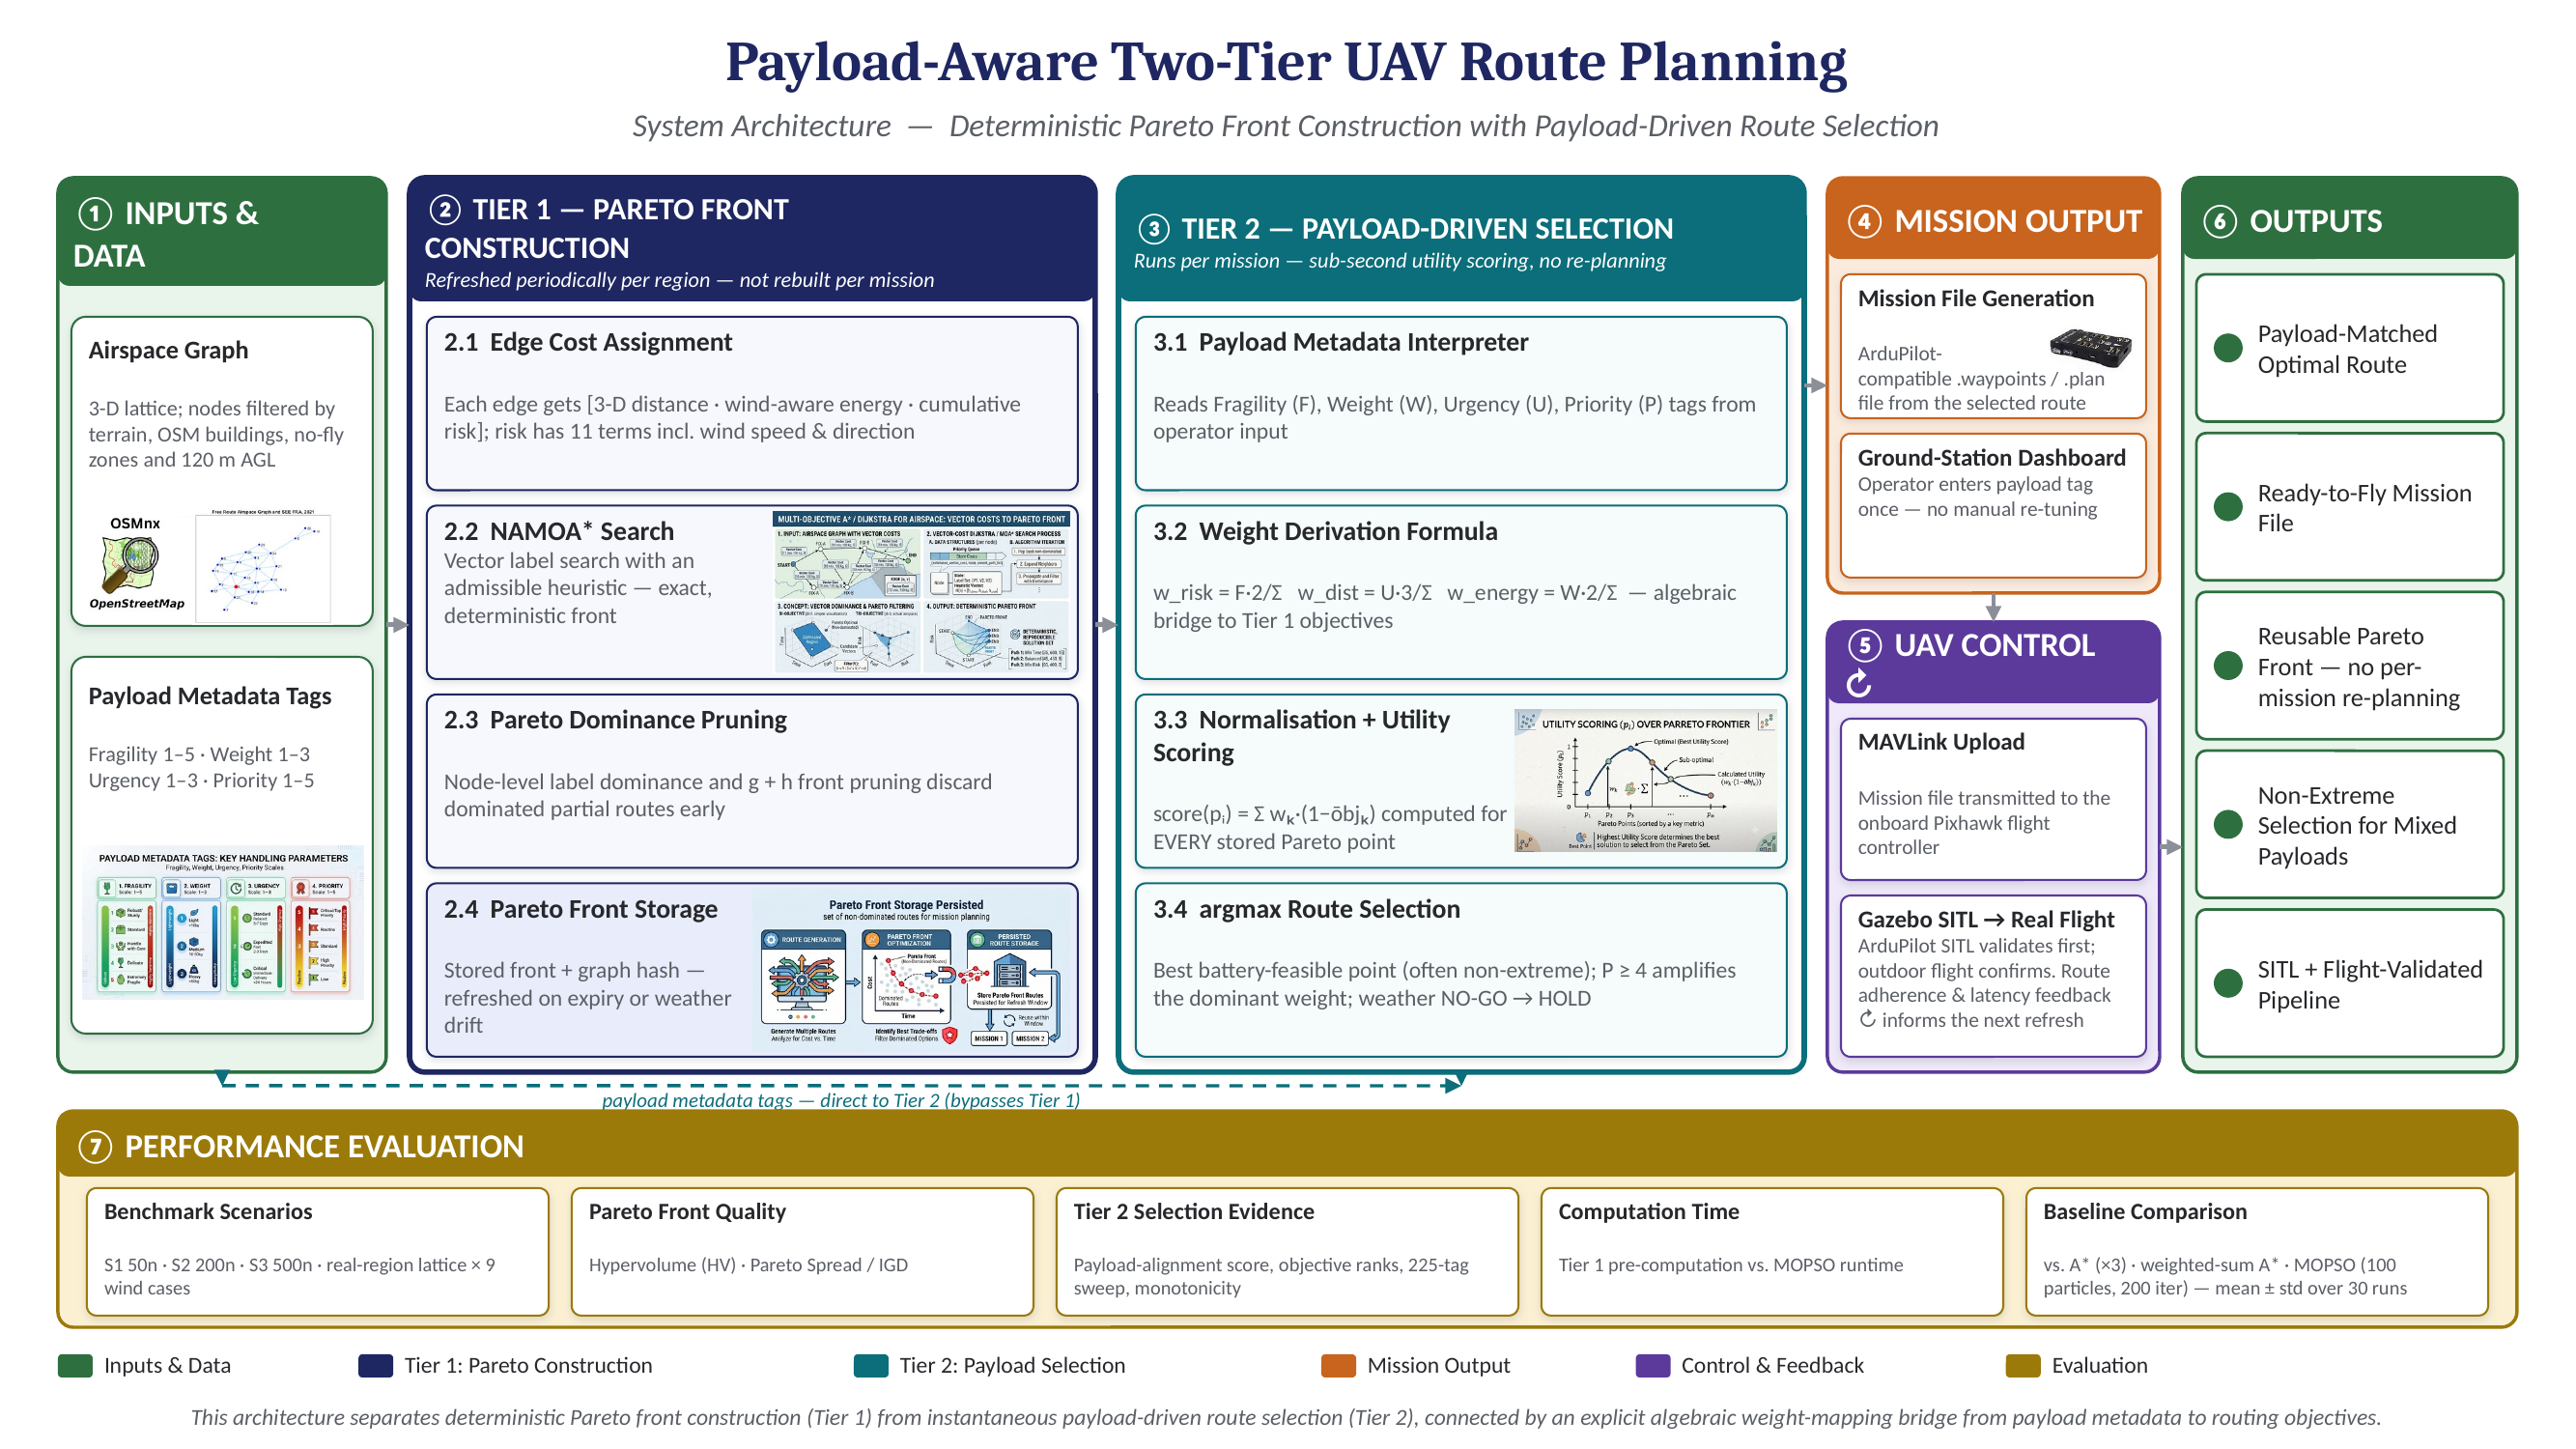
\includegraphics[width=\linewidth,height=0.62\textheight,keepaspectratio]{fig4_1_methodology_overview.png}
    \figcap{Fig. 4.1 -- Methodology overview: Tier 1 front construction feeding Tier 2 route selection}
  \end{minipage}\hfill
  \begin{minipage}[t]{0.41\textwidth}
    \centering
    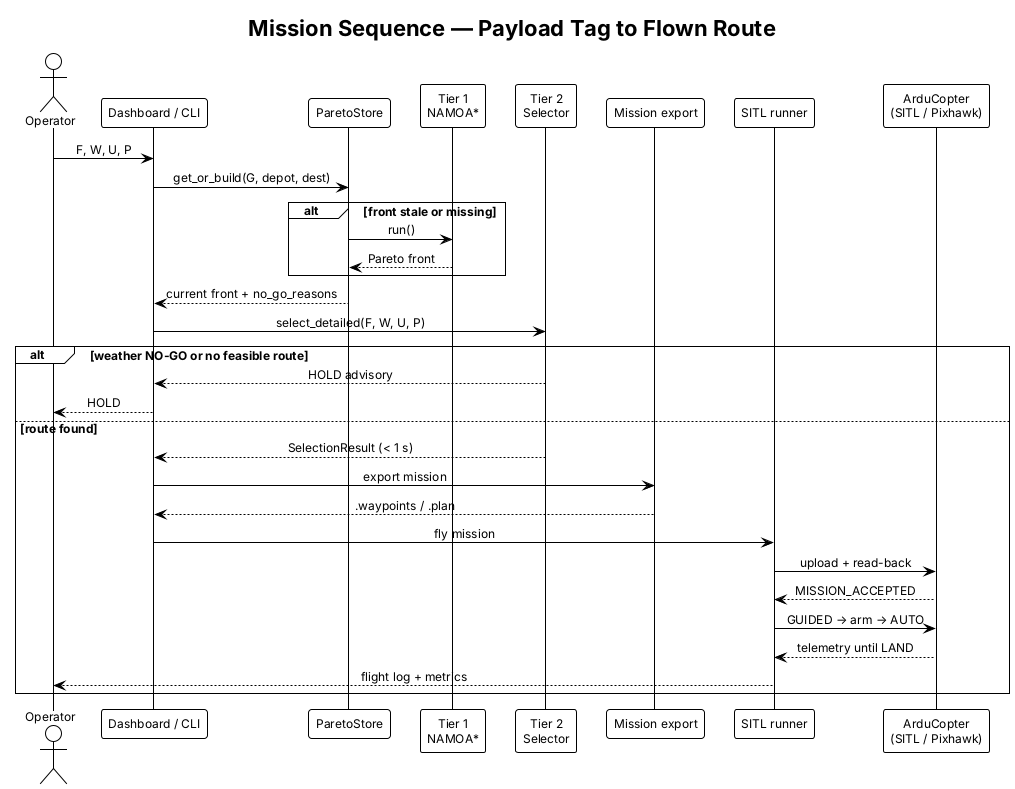
\includegraphics[width=\linewidth,height=0.62\textheight,keepaspectratio]{fig4_3_mission_sequence.png}
    \figcap{Fig. 4.3 -- Mission sequence from payload tag entry to the flown route}
  \end{minipage}
\end{frame}

% ======================================================================
% 14. Core algorithms
\begin{frame}{Core Algorithms --- NAMOA* \& Payload Selection}
  \compactblocks
  \scriptsize
  \begin{columns}[T,onlytextwidth]
    \column{0.47\textwidth}
      \begin{block}{Tier 1 --- NAMOA* (exact Pareto search)}
        \begin{itemize}
          \item One label (node, $g$, parent) per non-dominated partial path, held in a flat table --- no path copying
          \item Admissible vector heuristic $h(v) = [h, h, 0]$, $h$ = great-circle distance to target
          \item A label is pruned when the current front weakly dominates $g + h$
          \item Reports a truncation flag + expansion/generation diagnostics if a search cap is hit
          \item Guarantees: IGD = 0 on every tested scenario --- the front contains every reference point
        \end{itemize}
      \end{block}
    \column{0.47\textwidth}
      \begin{block}{Tier 2 --- Payload-Driven Selection}
        \begin{itemize}
          \item $r_{\text{raw}} = F\times 2$,\; $d_{\text{raw}} = U\times 3$,\; $e_{\text{raw}} = W\times 2$ $\rightarrow$ normalised into $w_{\text{risk}}, w_{\text{dist}}, w_{\text{energy}}$
          \item High priority ($P_{\text{lvl}} \ge 4$): dominant weight amplified by $0.1\times w_{\max}$, then renormalised
          \item Min-max normalise every route's $(d, \varepsilon, \rho)$ across the front
          \item $\mathrm{score}(p) = w_{\text{dist}}(1-\tilde d) + w_{\text{energy}}(1-\tilde\varepsilon) + w_{\text{risk}}(1-\tilde\rho)$;\; $p^* = \arg\max\, \mathrm{score}$
          \item Battery-infeasible routes removed first; weather HOLD returned if no route survives
        \end{itemize}
      \end{block}
  \end{columns}
  \vspace{4mm}

  \setlength{\statheight}{1.0cm}%
  \renewcommand{\statvalue}{\large}%
  \centering
  \stat[0.27\textwidth]{$<$ 1 ms}{Tier 2 selection latency (target was $<$ 1 s)}\hspace{5mm}%
  \stat[0.27\textwidth]{IGD = 0}{NAMOA* front vs.\ reference, every scenario}\hspace{5mm}%
  \stat[0.27\textwidth]{0 / 225}{monotonicity violations across the full tag sweep}
\end{frame}

% ======================================================================
% 15. Activity flows
\begin{frame}{Tier 1 \& Tier 2 Activity Flows}
  \centering
  \begin{minipage}[t]{0.32\textwidth}
    \centering
    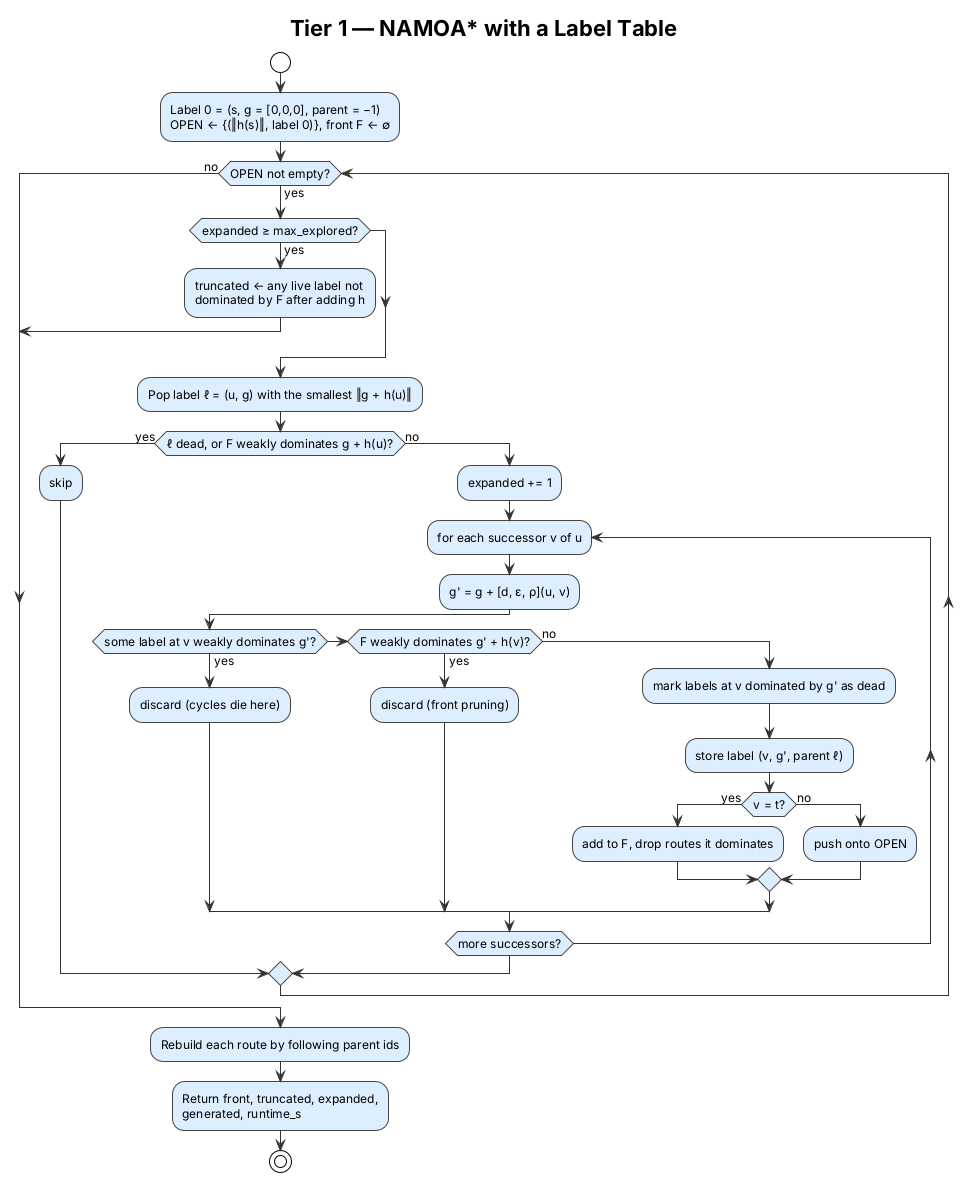
\includegraphics[width=\linewidth,height=0.64\textheight,keepaspectratio]{fig4_7_tier1_namoa.png}
    \figcap{Fig. 4.7 -- Tier 1: NAMOA* with a label table}
  \end{minipage}\hfill
  \begin{minipage}[t]{0.32\textwidth}
    \centering
    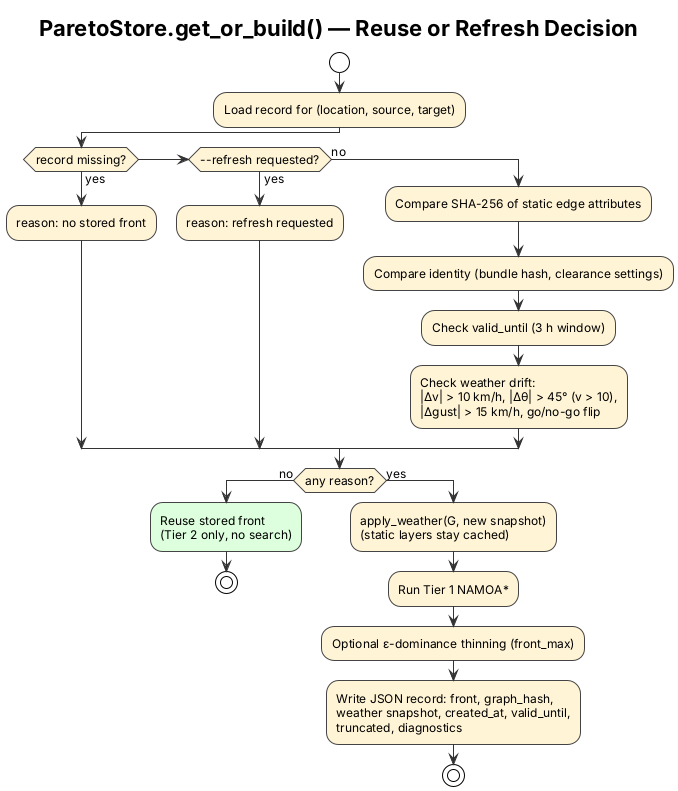
\includegraphics[width=\linewidth,height=0.64\textheight,keepaspectratio]{fig4_8_front_store.png}
    \figcap{Fig. 4.8 -- Front store: reuse or rebuild}
  \end{minipage}\hfill
  \begin{minipage}[t]{0.32\textwidth}
    \centering
    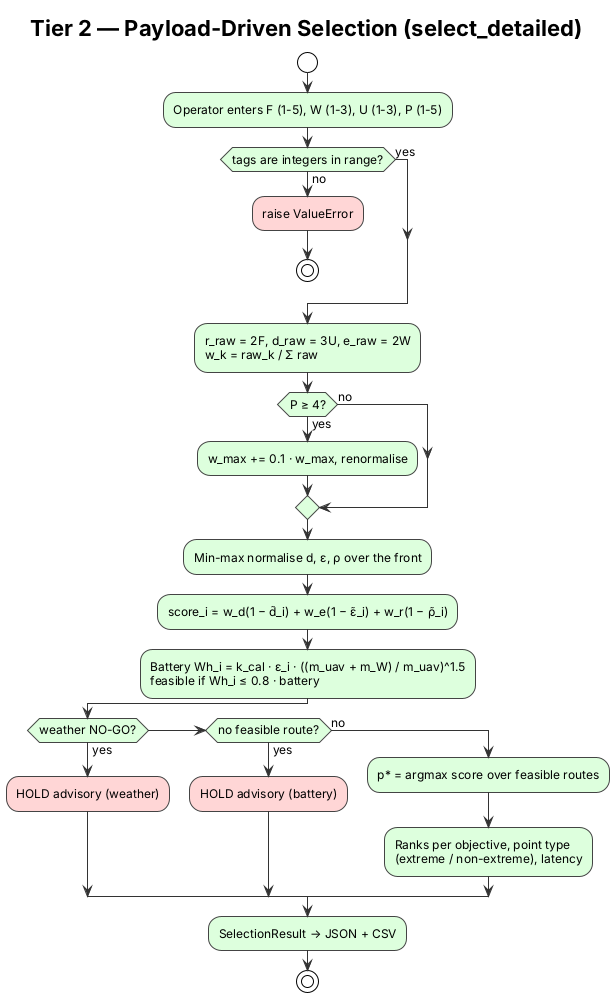
\includegraphics[width=\linewidth,height=0.64\textheight,keepaspectratio]{fig4_9_tier2_flow.png}
    \figcap{Fig. 4.9 -- Tier 2: validation, feasibility, weather hold}
  \end{minipage}
\end{frame}

% ======================================================================
% 16. Payload metadata -> weights
\begin{frame}{Payload Metadata $\rightarrow$ Routing Weights}
  \footnotesize
  Each of the four payload tags maps to exactly one Tier 1 objective --- a deterministic algebraic bridge, not an expert-set rule:
  \vspace{2mm}

  \begin{columns}[c,onlytextwidth]
    \column{0.55\textwidth}
      \centering
      \scriptsize
      \begin{tabularx}{\linewidth}{>{\raggedright\arraybackslash}p{2.3cm} >{\centering\arraybackslash}p{1.3cm} X}
        \toprule
        \textbf{Payload tag} & \textbf{Maps to} & \textbf{Reasoning} \\
        \midrule
        Fragility ($F$), 1--5 & $w_{\text{risk}}$ & Fragile items need low-vibration, low-risk corridors \\
        Payload weight ($W$), 1--3 & $w_{\text{energy}}$ & Heavier payload $\rightarrow$ higher hover/lift power draw \\
        Delivery urgency ($U$), 1--3 & $w_{\text{dist}}$ & Time-critical deliveries need the shortest path \\
        Priority level ($P_{\text{lvl}}$), 1--5 & amplifier & Scales the dominant weight when scores are close \\
        \bottomrule
      \end{tabularx}
    \column{0.42\textwidth}
      \begin{block}{Reference presets \& derived weights}
        \scriptsize
        \centering
        \begin{tabularx}{\linewidth}{>{\raggedright\arraybackslash}X ccc}
          \toprule
          \textbf{Preset} & $w_{\text{risk}}$ & $w_{\text{dist}}$ & $w_{\text{energy}}$ \\
          \midrule
          Fragile medical    & 0.667 & 0.200 & 0.133 \\
          Emergency medicine & 0.144 & 0.712 & 0.144 \\
          Disaster relief    & 0.182 & 0.273 & 0.545 \\
          Mixed cargo        & 0.375 & 0.375 & 0.250 \\
          \bottomrule
        \end{tabularx}
        \vspace{2mm}

        \raggedright
        Only emergency medicine has $P_{\text{lvl}} \ge 4$, so it is the only preset whose dominant weight (distance) is amplified.
      \end{block}
  \end{columns}
\end{frame}

% ======================================================================
% 17. Implementation status
\begin{frame}{Implementation Status}
  \scriptsize
  \renewcommand{\arraystretch}{0.95}%
  \begin{tabularx}{\textwidth}{>{\raggedright\arraybackslash}p{3.6cm}>{\centering\arraybackslash}p{2.9cm}X}
    \toprule
    \textbf{Module} & \textbf{Status} & \textbf{Evidence} \\
    \midrule
    1 --- Airspace Graph Builder & Complete & Lattice + cost pipeline running on real \& synthetic graphs \\
    2 --- Tier 1 NAMOA* & Complete & Front equals brute-force front on small graphs; 0 dominated/duplicate routes \\
    3 --- Baseline Planners & Complete & 3$\times$ A*, weighted-sum A*, MOPSO implemented and run \\
    4 --- Tier 2 Selector & Complete & Weight bridge, feasibility filter, weather HOLD, JSON/CSV record \\
    5 --- Evaluation Suite & Complete (1st pass) & HV/IGD/spread, 225-tag sweep, ablation --- report-scale run in progress \\
    6 --- Mission Export \& Dashboard & Complete (2 open defects) & QGC WPL 110 export verified by round-trip test; Tkinter dashboard functional \\
    7 --- Simulation \& SITL & Core flown, fidelity pending & SITL mission chain verified; Gazebo wind \& battery calibration next \\
    \bottomrule
  \end{tabularx}
  \vspace{2mm}

  \setlength{\statheight}{0.95cm}%
  \renewcommand{\statvalue}{\large}%
  \centering
  \stat[0.27\textwidth]{$\sim$265}{automated tests (planner + simulation suites)}\hspace{5mm}%
  \stat[0.27\textwidth]{0.11--0.13 m}{cross-track RMS error, flown vs.\ planned route in SITL}\hspace{5mm}%
  \stat[0.27\textwidth]{Oct--Dec}{remaining benchmarking + simulation-fidelity cycle}
\end{frame}

% ======================================================================
% 18. Simulation pipeline & classes
\begin{frame}{Simulation Pipeline \& Core Classes}
  \centering
  \begin{minipage}[t]{0.30\textwidth}
    \centering
    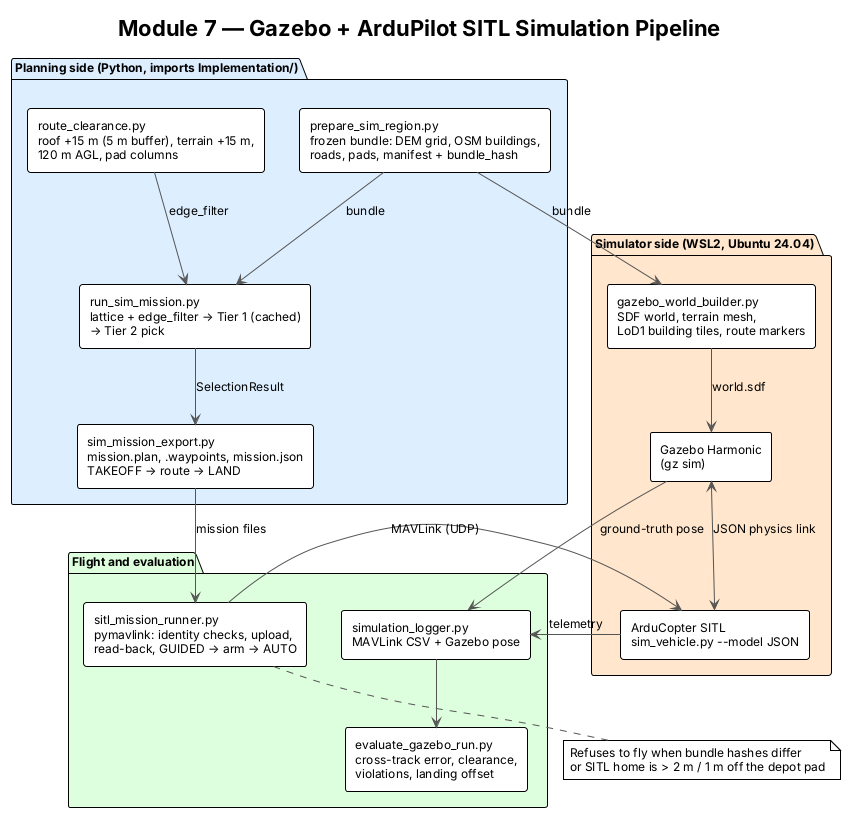
\includegraphics[width=\linewidth,height=0.55\textheight,keepaspectratio]{fig4_10_sim_pipeline.png}
    \figcap{Fig. 4.10 -- Gazebo and ArduPilot SITL simulation pipeline}
  \end{minipage}\hfill
  \begin{minipage}[t]{0.67\textwidth}
    \centering
    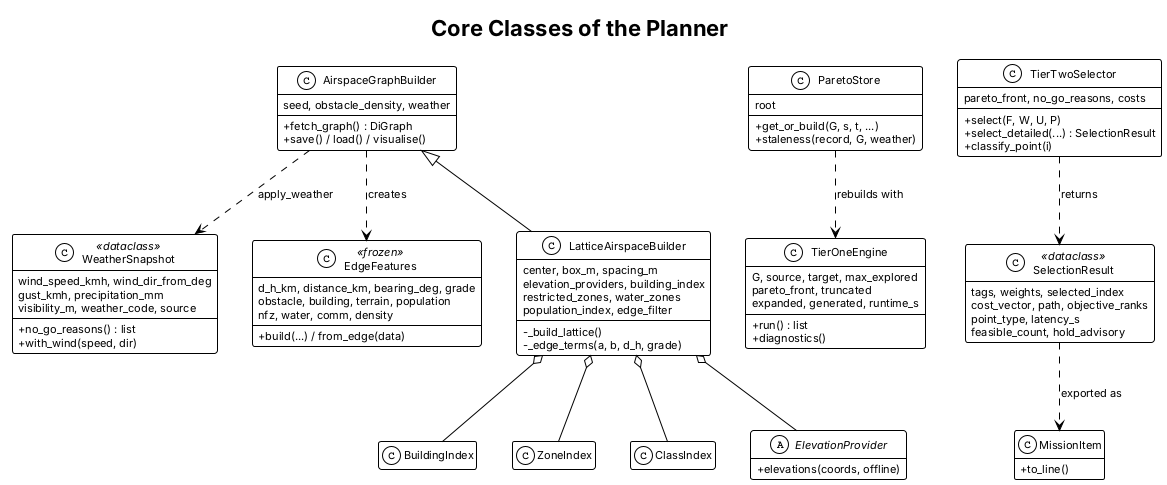
\includegraphics[width=\linewidth,height=0.55\textheight,keepaspectratio]{fig5_1_core_classes.png}
    \figcap{Fig. 5.1 -- Core classes of the planner}
  \end{minipage}
\end{frame}

% ======================================================================
% 19. Results: Tier 1 front quality
\begin{frame}{Results --- Tier 1 Front Quality vs.\ Baselines}
  \compactblocks
  \begin{columns}[T,onlytextwidth]
    \column{0.52\textwidth}
      \centering
      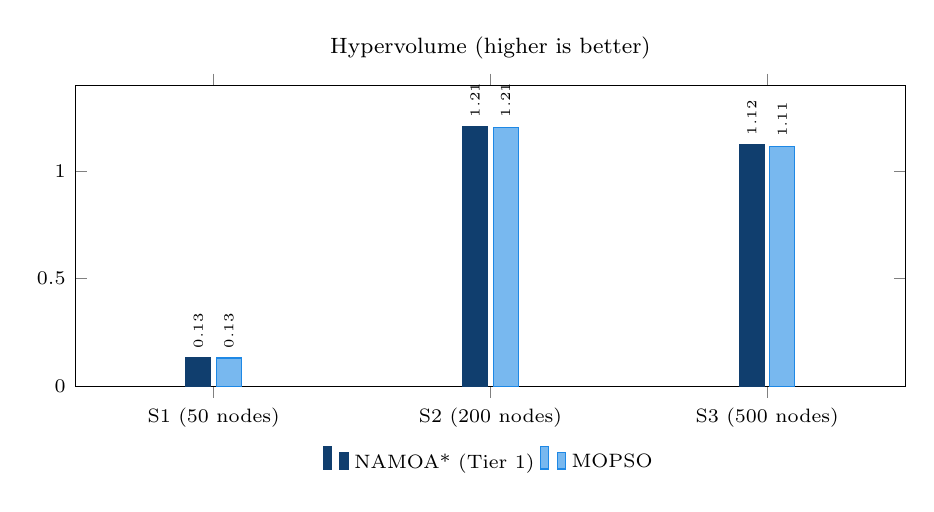
\begin{tikzpicture}
        \begin{axis}[
            title={\footnotesize Hypervolume (higher is better)},
            ybar, bar width=9pt,
            width=\linewidth, height=5.4cm,
            ymin=0, ymax=1.4,
            symbolic x coords={S1 (50 nodes),S2 (200 nodes),S3 (500 nodes)},
            xtick=data,
            tick label style={font=\scriptsize},
            nodes near coords,
            nodes near coords style={font=\tiny,rotate=90,anchor=west},
            legend style={font=\scriptsize,at={(0.5,-0.18)},anchor=north,legend columns=2,draw=none},
            enlarge x limits=0.25]
          \addplot[fill=UniversityBlue,draw=UniversityBlue] coordinates
            {(S1 (50 nodes),0.131) (S2 (200 nodes),1.2065) (S3 (500 nodes),1.1235)};
          \addplot[fill=AccentBlue!60,draw=AccentBlue] coordinates
            {(S1 (50 nodes),0.131) (S2 (200 nodes),1.2061) (S3 (500 nodes),1.1146)};
          \legend{NAMOA* (Tier 1), MOPSO}
        \end{axis}
      \end{tikzpicture}
    \column{0.45\textwidth}
      \begin{block}{What the exact IGD = 0 result means}
        \scriptsize
        \begin{itemize}
          \item NAMOA* front contains every point of the reference front on every scenario (IGD = 0)
          \item MOPSO recovers only 12 of 16 routes on S2, and 38 of 115 on S3
          \item HV gap stays small (0.0004 on S2, 0.009 on S3) because MOPSO still spans the extremes
          \item Missed interior points are exactly what Tier 2 needs for mixed payloads
          \item Cost of exactness: 33.8 s (NAMOA*) vs.\ 4.3 s (MOPSO) on S3 --- acceptable since Tier 1 runs once per region/weather window, not per mission
        \end{itemize}
      \end{block}
  \end{columns}
  \vspace{2mm}

  {\footnotesize\textbf{Bottom line: the exact method wins on front coverage and spread, where it matters for payload-aware selection --- not just on the headline HV number.}}
\end{frame}

% ======================================================================
% 20. Results: wind direction
\begin{frame}{Results --- Effect of Wind Direction on the Front}
  \compactblocks
  \begin{columns}[T,onlytextwidth]
    \column{0.54\textwidth}
      \centering
      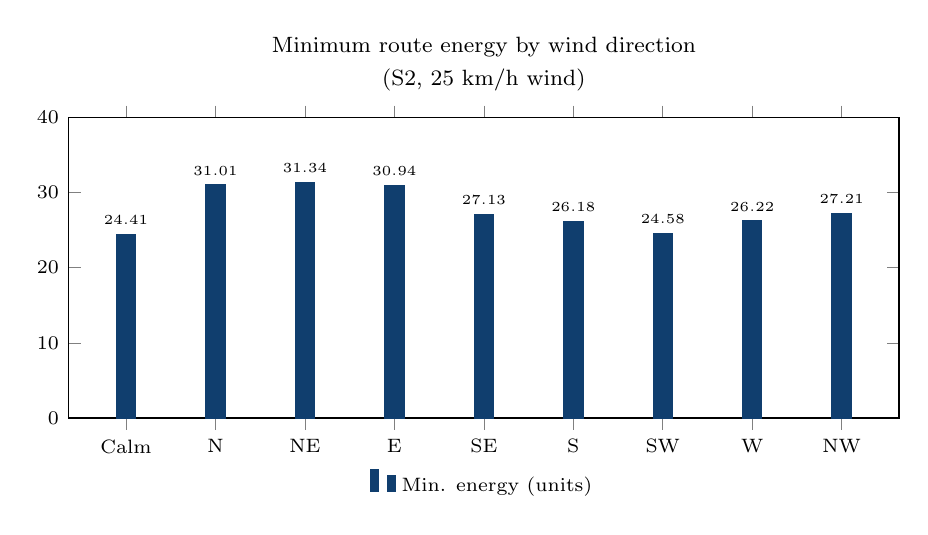
\begin{tikzpicture}
        \begin{axis}[
            title={\footnotesize Minimum route energy by wind direction\\\footnotesize (S2, 25 km/h wind)},
            title style={align=center},
            ybar, bar width=7pt,
            width=\linewidth, height=5.4cm,
            ymin=0, ymax=40,
            symbolic x coords={Calm,N,NE,E,SE,S,SW,W,NW},
            xtick=data,
            tick label style={font=\scriptsize},
            nodes near coords,
            nodes near coords style={font=\tiny,/pgf/number format/fixed,/pgf/number format/precision=2},
            legend style={font=\scriptsize,at={(0.5,-0.15)},anchor=north,draw=none},
            enlarge x limits=0.08]
          \addplot[fill=UniversityBlue,draw=UniversityBlue] coordinates
            {(Calm,24.41) (N,31.01) (NE,31.34) (E,30.94) (SE,27.13) (S,26.18) (SW,24.58) (W,26.22) (NW,27.21)};
          \legend{Min. energy (units)}
        \end{axis}
      \end{tikzpicture}
    \column{0.43\textwidth}
      \begin{block}{Why direction --- not just speed --- matters}
        \scriptsize
        \begin{itemize}
          \item Same wind speed: cheapest route needs 24.58 energy units (SW wind) vs.\ 31.34 (NE wind) --- a 27.5\% swing
          \item Opposite directions give the same minimum risk (crosswind depends only on the wind's axis) but very different minimum energy (headwind depends on direction along that axis)
          \item East-bound edges cost 27.8\% more energy/km than west-bound edges under an east wind
          \item N--S edges carry 6$\times$ the crosswind risk of E--W edges (0.225 vs.\ 0.038)
        \end{itemize}
      \end{block}
  \end{columns}
  \vspace{2mm}

  {\scriptsize\textbf{Open question for the next pass: under steady wind, three of four payload presets converge on the same route on the benchmark graph --- is that the right answer, or an artefact of min-max normalisation on a short front?}}
\end{frame}

% ======================================================================
% 21. Ablation
\begin{frame}{Contribution of Each Risk Layer (Ablation)}
  \begin{columns}[T,onlytextwidth]
    \column{0.40\textwidth}
      \centering
      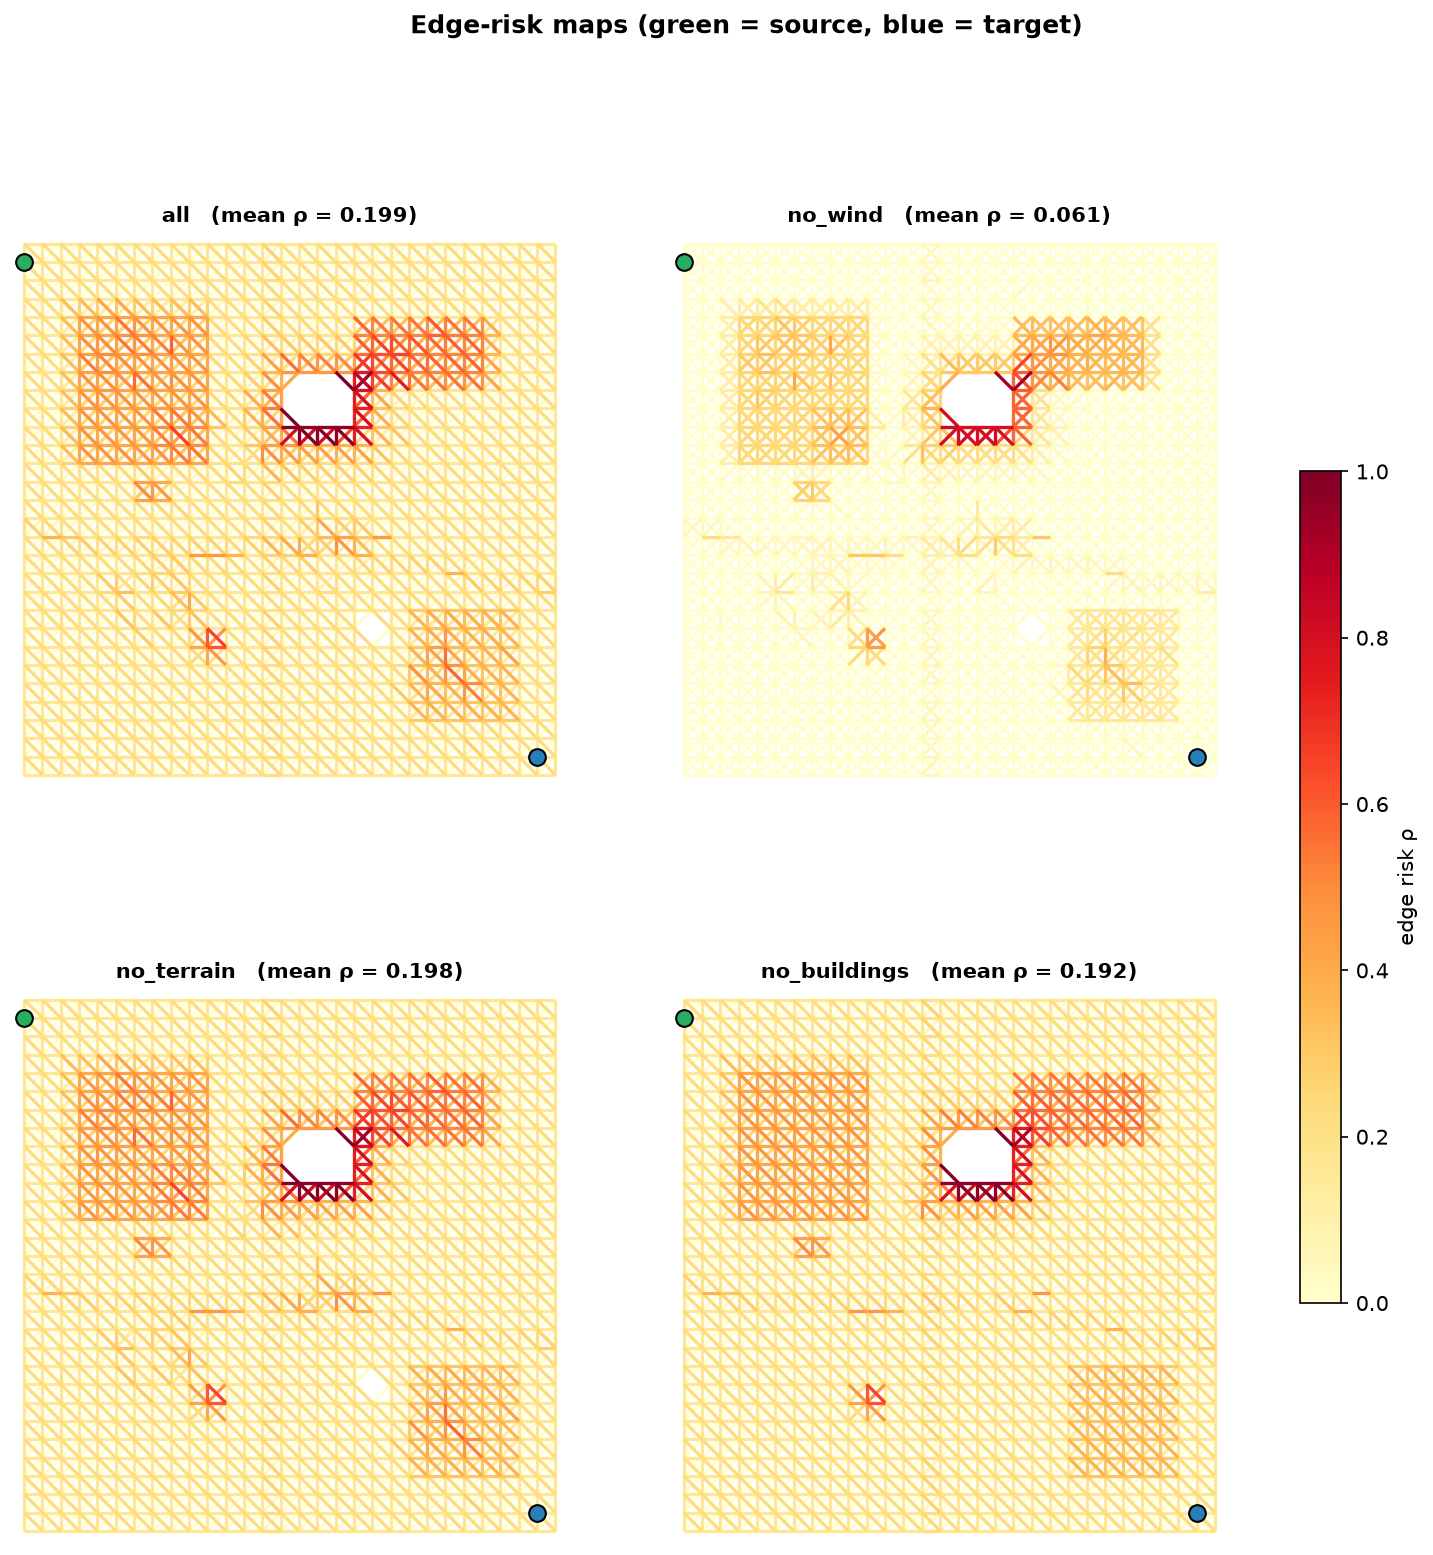
\includegraphics[width=\linewidth,height=0.66\textheight,keepaspectratio]{fig6_4_ablation_risk_maps.png}
      \figcap{Fig. 6.4 -- Edge risk maps for the ablation variants (fixture layers)}
    \column{0.57\textwidth}
      \small
      \textbf{Table 6.5 -- 30 km/h wind from SW, 6 km lattice}
      \vspace{1mm}

      \footnotesize
      \begin{itemize}
        \setlength{\itemsep}{1.5mm}
        \item All layers: 196 routes, mean edge risk 0.199
        \item No wind: 205 routes, mean edge risk 0.061 ($-69\%$); safest route risk drops from 8.85 to 0.10
        \item No terrain: only 56 routes --- altitude changes are what separate otherwise similar paths
        \item No buildings: 190 routes, higher max risk (13.08 $\rightarrow$ 12.26 removed)
        \item Wind is the single largest driver of risk; terrain mostly drives front size; buildings raise the upper end of the risk range
      \end{itemize}
  \end{columns}
\end{frame}

% ======================================================================
% 22. Tier 2 results & simulation
\begin{frame}{Results --- Tier 2 Selection \& Simulation}
  \compactblocks
  \begin{columns}[T,onlytextwidth]
    \column{0.56\textwidth}
      \scriptsize
      \setlength{\tabcolsep}{4pt}%
      \begin{tabularx}{\linewidth}{>{\raggedright\arraybackslash}X *{3}{>{\centering\arraybackslash}p{0.9cm}} >{\centering\arraybackslash}p{1.6cm}}
        \toprule
        \textbf{Preset (S3, 115-route front)} & \textbf{Rank: dist} & \textbf{Rank: energy} & \textbf{Rank: risk} & \textbf{Point type} \\
        \midrule
        Fragile medical    & 91 & 81 & 25 & non-extreme \\
        Emergency medicine & 22 & 26 & 94 & non-extreme \\
        Disaster relief    & 28 & 1  & 88 & min-energy \\
        Mixed cargo        & 84 & 59 & 32 & non-extreme \\
        \bottomrule
      \end{tabularx}
      \vspace{1.5mm}

      \scriptsize
      All four presets pick four different, mostly non-extreme routes on the large front --- trade-offs a single-objective or fixed-weight planner cannot make.
      \vspace{2.5mm}

      \setlength{\statheight}{1.6cm}%
      \renewcommand{\statvalue}{\large}%
      \noindent
      \stat[\dimexpr0.5\linewidth-0.6em-8pt\relax]{1.9\%}{longer than the shortest route --- emergency medicine's pick, for a much lower risk}\hfill
      \stat[\dimexpr0.5\linewidth-0.6em-8pt\relax]{$<$1 ms}{every Tier 2 selection, far inside the 1 s target}
    \column{0.41\textwidth}
      \begin{block}{Simulation (Gazebo + ArduPilot SITL)}
        \scriptsize
        \begin{itemize}
          \item Mission upload, read-back, switch to AUTO, landing and disarm all succeeded
          \item Cross-track RMS error: 0.11--0.13 m
          \item Landing offset from destination pad: 0.01--0.02 m
          \item Confirms the mission chain from Tier 2 to the autopilot is correct, including the altitude frame
          \item Not yet covered: the 3-D city model, wind in the simulator, and calibrated battery constants
        \end{itemize}
      \end{block}
  \end{columns}
\end{frame}

% ======================================================================
% 23. Tier 2 routes & SITL screenshot
\begin{frame}{Tier 2 Routes on the Lattice \& SITL Simulation (Fig. 6.5)}
  \centering
  \begin{minipage}[t]{0.34\textwidth}
    \centering
    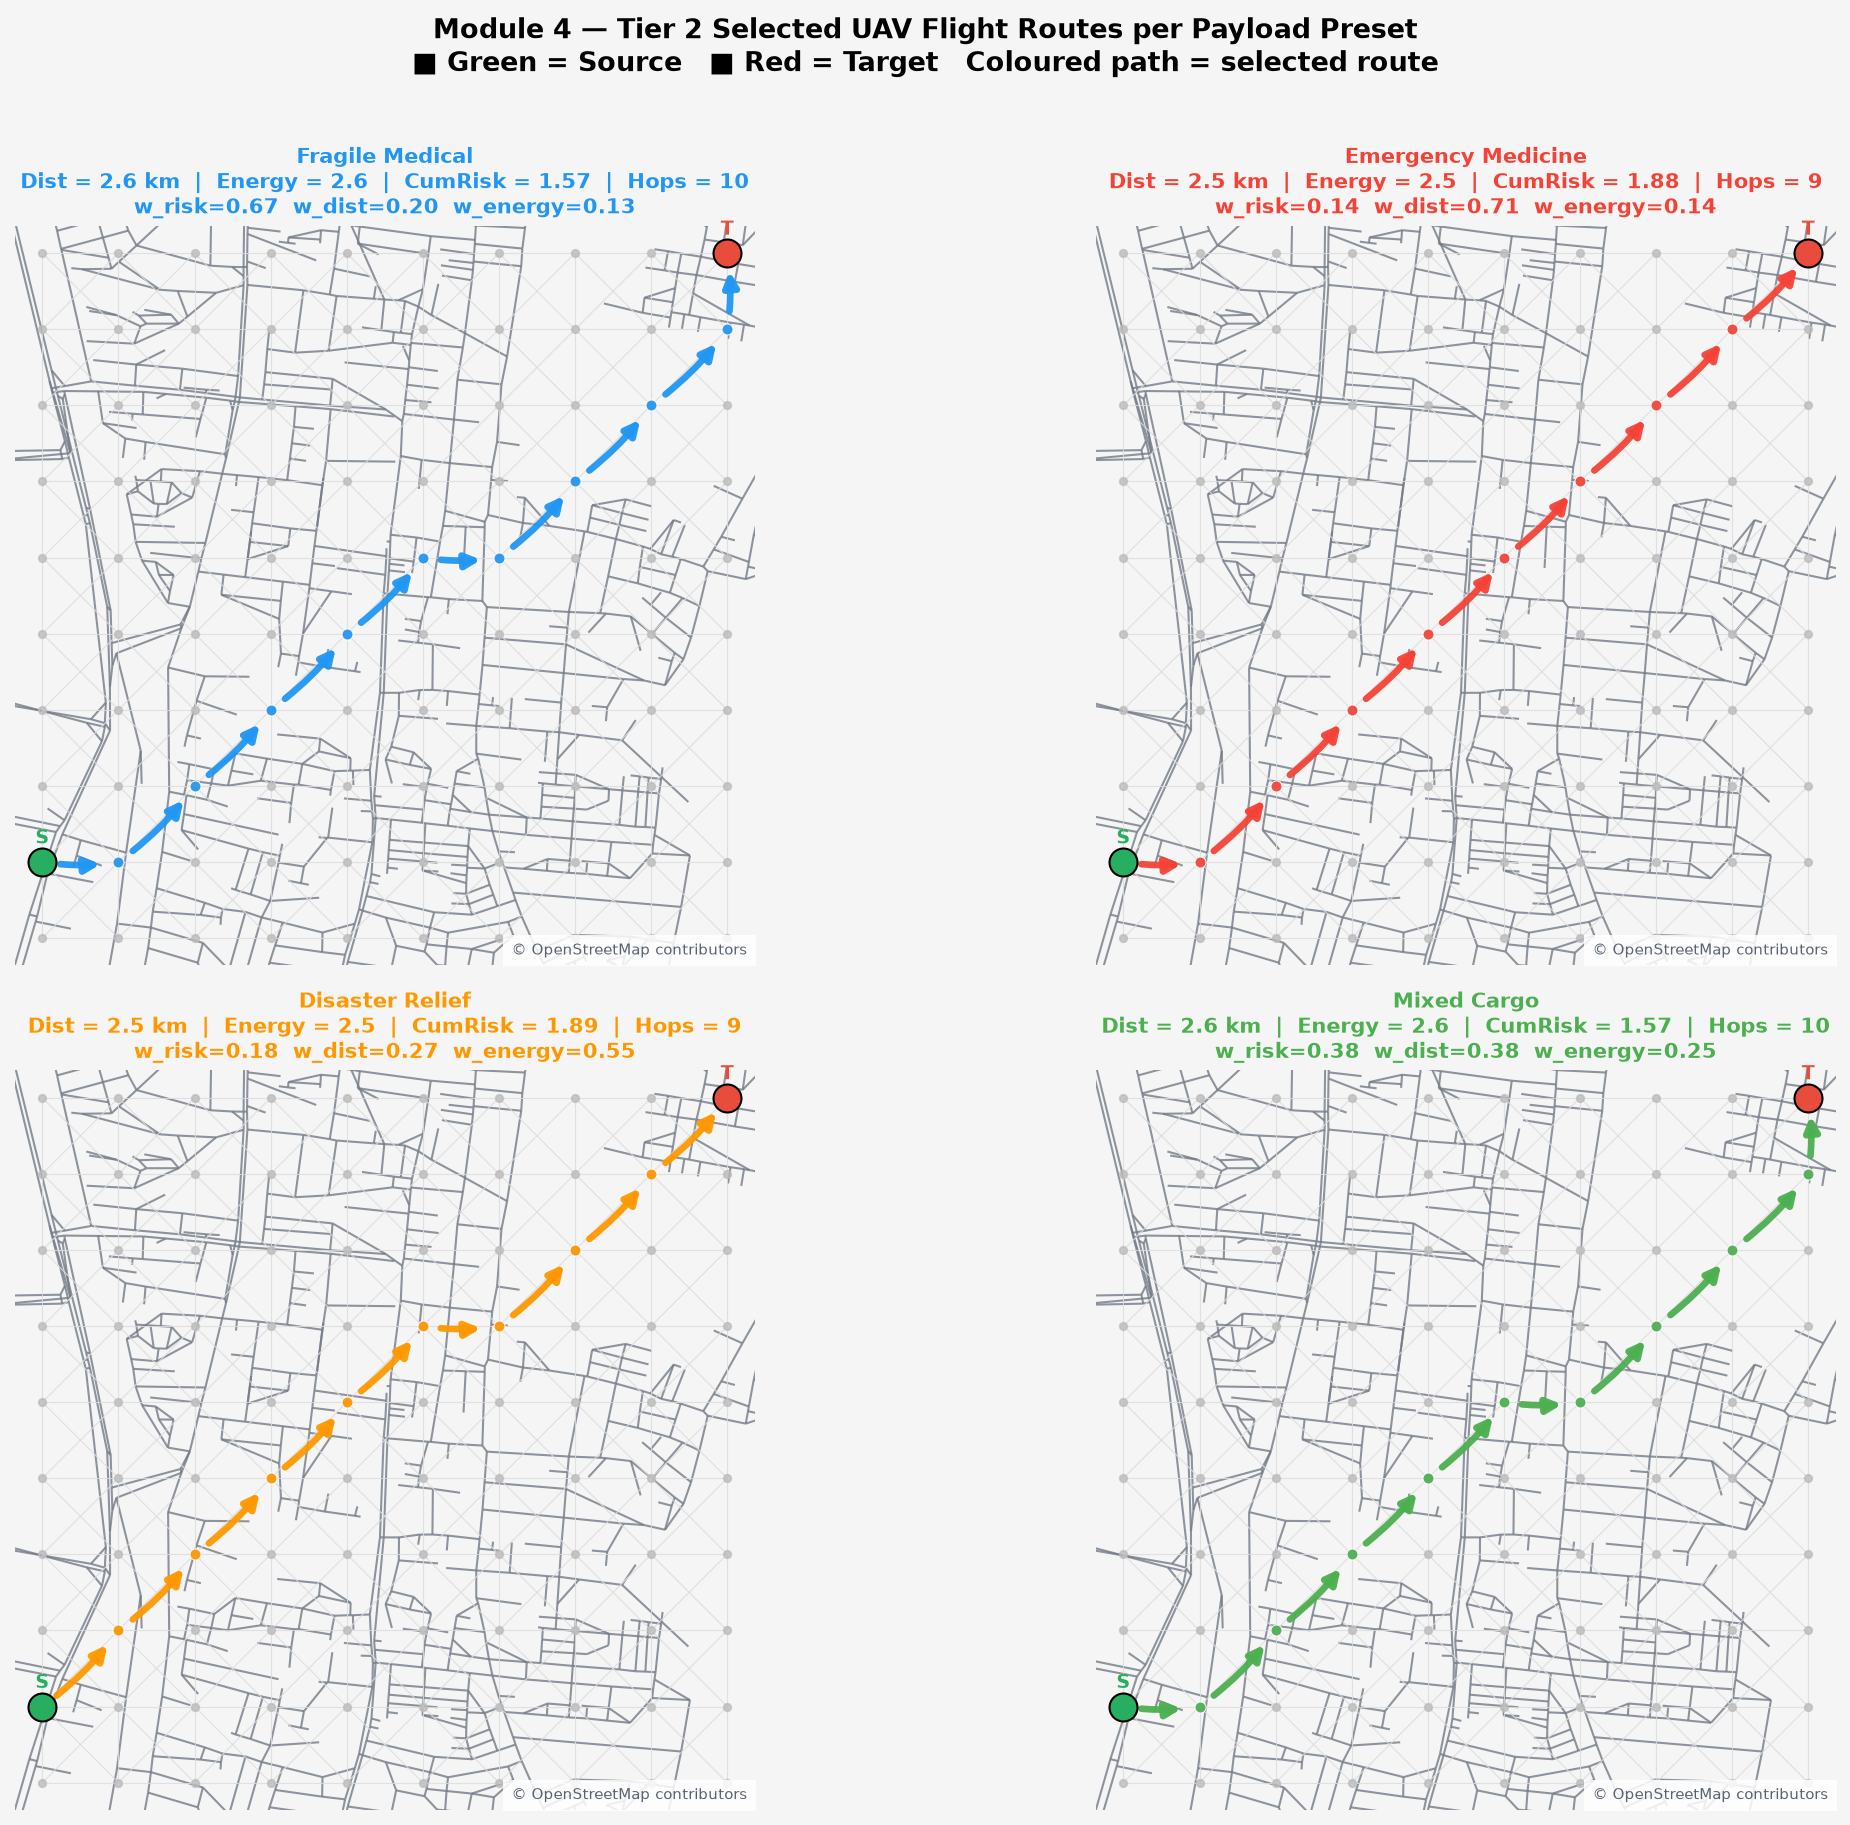
\includegraphics[width=\linewidth,height=0.60\textheight,keepaspectratio]{fig6_5_tier2_routes.png}
    \figcap{Fig. 6.5 -- Tier 2 routes for the four presets on a 2 km lattice}
  \end{minipage}\hfill
  \begin{minipage}[t]{0.63\textwidth}
    \centering
    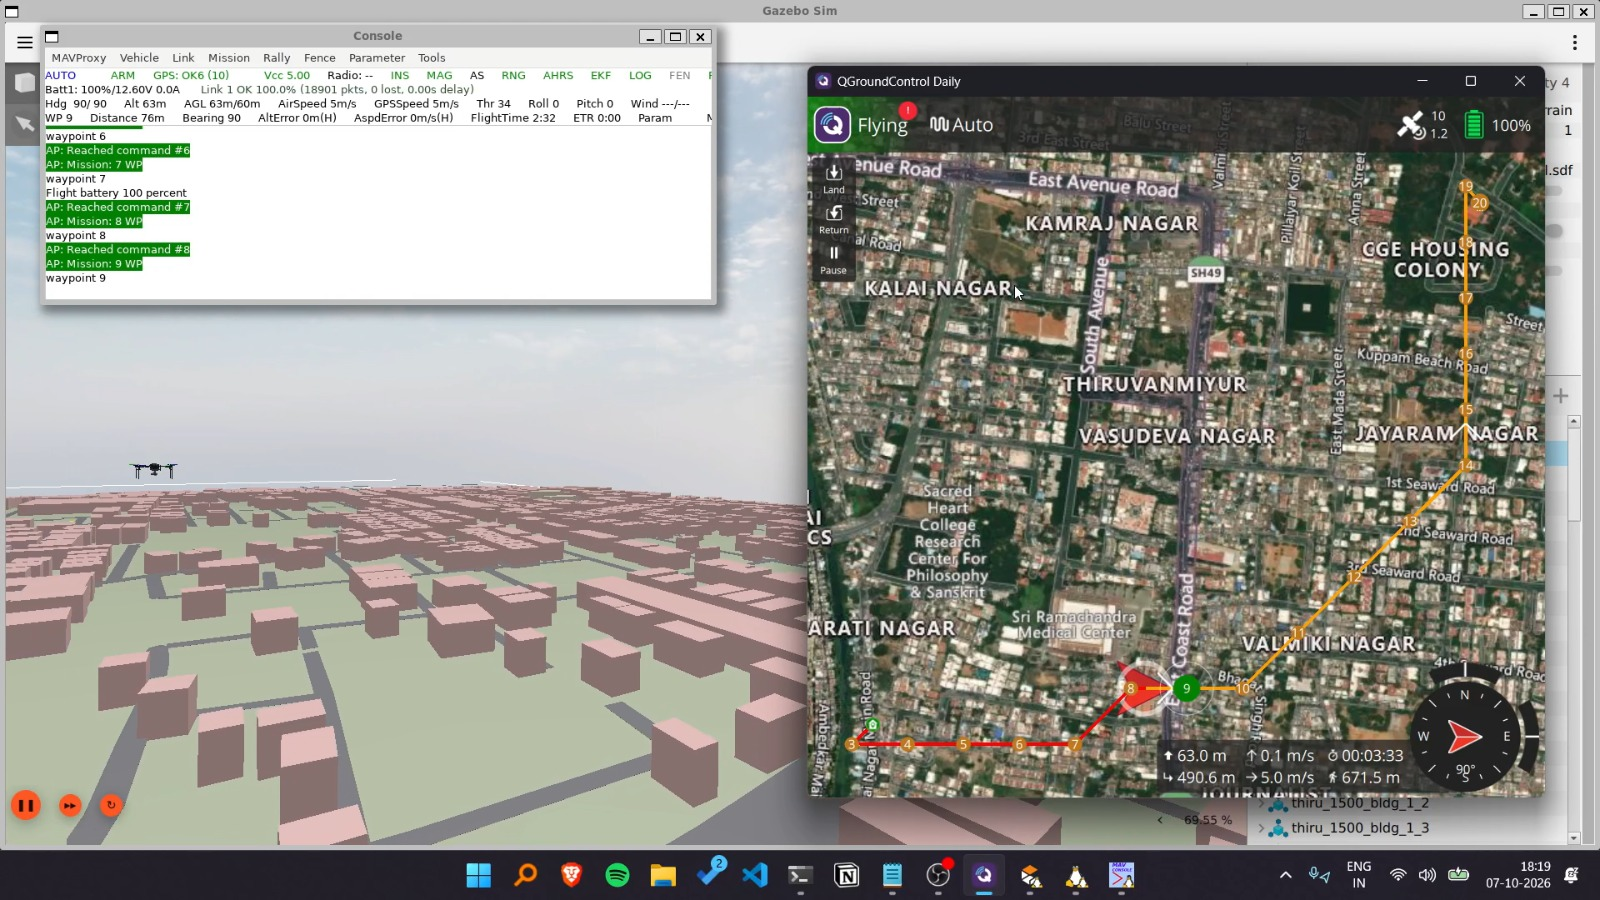
\includegraphics[width=\linewidth,height=0.60\textheight,keepaspectratio]{sitl_gazebo_screenshot.jpg}
    \figcap{Gazebo Harmonic + ArduPilot SITL flying an uploaded Tier 2 mission in AUTO --- MAVProxy console (left), QGroundControl mission replay (right)}
  \end{minipage}
\end{frame}

% ======================================================================
% 24. Comparison with existing work
\begin{frame}{Comparison with Existing Work}
  \scriptsize
  \begin{tabularx}{\textwidth}{>{\raggedright\arraybackslash}p{2.3cm} >{\raggedright\arraybackslash}X >{\raggedright\arraybackslash}X >{\raggedright\arraybackslash}X >{\raggedright\arraybackslash\bfseries}X}
    \toprule
    \textbf{Property} & \textbf{Chokkalingam \& Ganesan} & \textbf{Tsoutsouras et al.} & \textbf{Ren et al.} & This Work \\
    \midrule
    Front construction & POPSO (stochastic) & None & CDNSGA-II (stochastic) & NAMOA* --- exact, deterministic \\
    Final selection & Weighted sum, re-tuned per mission & Not applicable & Crowding distance & Utility from payload tags, argmax over full front \\
    Payload in selection & No & Mass in energy model only & No & Fragility, weight, urgency, priority \\
    Wind direction in cost & Not reported & Not reported & Not reported & Headwind + crosswind per edge, gust, weather gate \\
    Front reuse & Re-run per mission & Not applicable & Re-run per mission & Stored front, drift-based refresh \\
    \bottomrule
  \end{tabularx}
  \vspace{4mm}

  \footnotesize
  The comparison is qualitative for the cited works (code/data not public); their selection rules (crowding distance, fixed weights) are applied to our fronts for the quantitative comparison, reported above with the payload-alignment metric.
\end{frame}

% ======================================================================
% 25. Discussion & next steps
\begin{frame}{Discussion \& Next Steps}
  \footnotesize
  \textbf{Supported so far}
  \begin{itemize}
    \item The exact Tier 1 front covers the reference front completely, while MOPSO recovers only a third of it on the largest scenario
    \item Tier 2 picks non-extreme routes for mixed payloads in well under a millisecond, and different payloads get different routes on a large front
    \item The directional wind model changes energy, risk and front shape as physics predicts --- a direction-blind model would miss a 27.5\% energy difference at a fixed wind speed
  \end{itemize}
  \vspace{2mm}

  \begin{block}{Next in the benchmark + simulation cycle}
    \begin{columns}[T,onlytextwidth]
      \column{0.49\textwidth}
        \begin{itemize}
          \item Run MOPSO at report-scale settings with per-repetition statistics
          \item Study the front collapse under steady wind (normalisation vs.\ weight multipliers)
          \item Calibrate risk weights and battery constants from simulated flights
        \end{itemize}
      \column{0.49\textwidth}
        \begin{itemize}
          \item Fix the density-label defect and re-group the monotonicity check by scenario
          \item Repeat ablation \& Tier 2 evaluation on live OpenStreetMap data
          \item Add wind to the Gazebo world; fly each preset under multiple wind cases
        \end{itemize}
    \end{columns}
  \end{block}
\end{frame}

% ======================================================================
% 26. Team responsibilities
\begin{frame}{Team Responsibilities}
  \scriptsize
  \begin{tabularx}{\textwidth}{>{\bfseries}p{2.6cm}>{\raggedright\arraybackslash}X >{\raggedright\arraybackslash}p{2.8cm}}
    \toprule
    Team Member & Responsibilities & Current Status \\
    \midrule
    Thirumurugan RA & Software simulation: Gazebo Harmonic world builder from OSM + DEM, ArduPilot SITL mission runner, QGC WPL 110 / .plan mission export, cross-track and landing-offset measurement, Gazebo wind and battery calibration & SITL chain verified; simulation fidelity in progress \\
    \addlinespace
    Meghna Manimaran & 3-D airspace lattice with multi-source node selection (DEM chain, OSM buildings, restricted zones, cached Overpass client), directional wind-aware energy and 11-component risk model, weather go/no-go gate, Tier 1 rewrite as NAMOA* with label table & Complete \\
    \addlinespace
    Shrika SP Thota & Front store with graph hash and weather-drift refresh, Tier 2 validation, battery feasibility and weather HOLD, baseline planners (A* $\times$3, weighted-sum A*, MOPSO), evaluation suite (HV, IGD, spread, 225-tag sweep, ablation), automated tests & First pass complete; report-scale run in progress \\
    \bottomrule
  \end{tabularx}
  \vspace{3mm}

  \scriptsize
  Phase I (through December) is a shared, coupled effort: the benchmarking/evaluation loop and the simulation-fidelity loop (Chapter 2) draw on all three members across weight calibration, baseline comparison and SITL validation.
\end{frame}

% ======================================================================
% 27. References
\begin{frame}{References}
  \scriptsize
  \begin{thebibliography}{9}
    \setlength{\itemsep}{0.6mm}
    \setlength{\parskip}{0pt}
    \bibitem{deng2026}
      J. Deng et al.,
      ``Multi-objective UAV trajectory planning algorithm based on the hybrid MS-INSGA2 strategy,''
      \emph{J. King Saud Univ. -- CIS}, 38(6), 2026.
    \bibitem{chokkalingam2026}
      K. Chokkalingam and R. Ganesan,
      ``Dynamic parameter adaptation in Pareto-optimal particle swarm optimization for efficient UAV path planning,''
      \emph{RAIRO -- OR}, 60(1), 2026.
    \bibitem{tsoutsouras2020}
      V. Tsoutsouras, J. Story, P. Stanley-Marbell,
      ``Payload-mass-aware trajectory planning on multi-user autonomous UAVs,''
      arXiv:2001.02531, 2020.
    \bibitem{oakey2021}
      A. Oakey et al.,
      ``Quantifying the effects of vibration on medicines in transit caused by fixed-wing and multi-copter drones,''
      \emph{Drones}, 5(1):22, 2021.
    \bibitem{stierlin2024}
      N. Stierlin et al.,
      ``Preanalytic integrity of blood samples in UAV medical transport: A comparative study,''
      \emph{Drones}, 8(9):517, 2024.
    \bibitem{deb2002}
      K. Deb, A. Pratap, S. Agarwal, T. Meyarivan,
      ``A fast and elitist multiobjective genetic algorithm: NSGA-II,''
      \emph{IEEE TEC}, 6(2), 2002.
    \bibitem{ren2019}
      Q. Ren, Y. Yao, G. Yang, X. Zhou,
      ``Multi-objective path planning for UAV in the urban environment based on CDNSGA-II,''
      \emph{IEEE SOSE}, 2019.
    \bibitem{dronerules2021}
      Ministry of Civil Aviation, Government of India,
      ``The Drone Rules, 2021,''
      Gazette of India, G.S.R. 589(E), 2021.
    \bibitem{openmeteo}
      Open-Meteo,
      ``Free weather API and elevation API,''
      open-meteo.com, 2026.
  \end{thebibliography}
\end{frame}

% ======================================================================
% 28. Thank you
\begin{frame}[plain]
  \centering
  \vfill
  {\usebeamerfont{title}\color{UniversityBlue}\Huge Thank You}\par
  
  \vfill
\end{frame}

\end{document}
